\documentclass[10pt, a4paper, oneside]{article}
\usepackage[hidelinks]{hyperref}
\usepackage{jucs2e}
\usepackage{graphicx}
\usepackage{url}
\usepackage{ulem}
\usepackage{mathtools}
\usepackage{algorithm} 
\usepackage{algpseudocode} 
\usepackage{scalerel}
\usepackage{setspace}
\usepackage[strict]{changepage}
\usepackage{caption}
\usepackage[letterspace=-50]{microtype}
\usepackage{fontspec}
\usepackage{afterpage}
\usepackage{ragged2e}

\setmainfont{Times New Roman}

\usepackage{titlesec}

\titleformat*{\section}{\Large\bfseries}
\titleformat*{\subsection}{\normalsize\bfseries}

\renewcommand{\baselinestretch}{0.9} 

\graphicspath{{./figures/}}

\usepackage[textwidth=8cm, margin=0cm, left=4.6cm, right=4.2cm, top=3.9cm, bottom=6.8cm, a4paper, headheight=0.5cm, headsep=0.5cm]{geometry}
\usepackage{fancyhdr}
\usepackage[format=plain, labelfont=it, textfont=it, justification=centering]{caption}
\usepackage{breakcites}
\usepackage{microtype}
 
\apptocmd{\frame}{}{\justifying}{}


\urlstyle{same}
\pagestyle{fancy}

\newcommand\jucs{{Journal of Universal Computer Science}}
\newcommand\jucsvol{vol. 31, no. 4 (2025)}
\newcommand\jucspages{363-382}
\newcommand\jucssubmitted{27/2/2024}
\newcommand\jucsaccepted{27/11/2024}
\newcommand\jucsappeared{28/3/2025}
\newcommand\jucslicence{ CC BY 4.0}
\newcommand\startingPage{363}
\setcounter{page}{\startingPage}

%Author
\newcommand\paperauthor{{Nhat P.M., Hien N.L.H., Toan D.M., Hung L.V., Binh P., Anh P.T., Phong N.T.H., Hieu N.V. }}

% Title
\newcommand\papertitle{EBAR: A Novel Machine Learning Model for Quantifying Chemical Concentrations using NIR Spectroscopy}

% Main header content
\header{\paperauthor \papertitle}

\begin{document}

\title{{\fontsize{14pt}{14pt}\selectfont{\vspace*{-3mm}\papertitle\vspace*{-1mm}}}}

\author{{\bfseries\fontsize{10pt}{10pt}\selectfont{Phan Minh Nhat}} \\
   {\fontsize{9pt}{12pt}\selectfont{(The University of Danang - University of Science and Technology, \city{Danang}, \country{Vietnam}, \\ \orcid{0009-0008-3861-9892},    nhat0299@gmail.com)}}
   \and
   {\bfseries\fontsize{10pt}{10pt}\selectfont{Ngo Le Huy Hien}}\\
   {\fontsize{9pt}{12pt}\selectfont{(Leeds Beckett University, \city{Leeds}, \city{England} \\
   \orcid{0000-0002-1439-8289}, 
   ngolehuyhien@gmail.com)}}
   \and
   {\bfseries\fontsize{10pt}{10pt}\selectfont{Dinh Minh Toan}}\\
   {\fontsize{9pt}{12pt}\selectfont{(The University of Danang - University of Science and Technology, \city{Danang}, \country{Vietnam}, \\ \orcid{0009-0000-3405-4638},    toandinh6501@gmail.com)}}
   \and
   {\bfseries\fontsize{10pt}{10pt}\selectfont{Le Viet Hung}}\\
   {\fontsize{9pt}{12pt}\selectfont{(The University of Danang - University of Science and Technology, \city{Danang}, \country{Vietnam}, \\ \orcid{0009-0007-5164-4761},    hungle.dut@gmail.com)}}
   \and
   {\bfseries\fontsize{10pt}{10pt}\selectfont{Phan Binh}}\\
   {\fontsize{9pt}{12pt}\selectfont{(The University of Danang - University of Science and Technology, \city{Danang}, \country{Vietnam}, \\ \orcid{0009-0002-8278-4218},    binhphan77373@gmail.com)}}
   \and
    {\bfseries\fontsize{10pt}{10pt}\selectfont{Phung Thi Anh}}\\
   {\fontsize{9pt}{12pt}\selectfont{(The University of Danang - University of Science and Technology, \city{Danang}, \country{Vietnam}, \\ \orcid{0009-0000-6018-2684},    anhhna17710110@gmail.com)}}
   \and
   {\bfseries\fontsize{10pt}{10pt}\selectfont{Nguyen Thi Hoang Phuong}}\\
   {\fontsize{9pt}{12pt}\selectfont{(Pham Van Dong University, QuangNgai, Viet Nam \\
   \orcid{0009-0009-6755-604X}, 
   nthphuong@pdu.edu.vn)}}
   \and
   {\bfseries\fontsize{10pt}{10pt}\selectfont{Nguyen Van Hieu}}\\
   {\fontsize{9pt}{12pt}\selectfont{(The University of Danang - University of Science and Technology, \city{Danang}, \country{Vietnam}, \\ \orcid{0000-0001-5311-806X},  
   nvhieuqt@dut.udn.vn)}}
}

\label{first}
\maketitle

{\fontfamily{ptm}\selectfont
\begin{abstract}
{\fontsize{9pt}{9pt}\selectfont{\vspace*{-2mm}
The examination of Near Infrared Reflectance Spectroscopy (NIR) in cattle and poultry fertilizers provides a viable solution for determining optimal fertilizer composition for crop growth while mitigating adverse impacts on soil and groundwater quality. In recent studies, conventional machine learning models combined with spectral analysis have been used to ascertain cattle and poultry fertilizer concentrations. However, these traditional machine learning models encounter challenges in achieving data generalization, resulting in suboptimal prediction accuracy. To address this issue, this study proposes a synthesized machine learning model named EBAR (Error Based Accumulation Regression), which exhibits a commendable coefficient of determination, with an average \(R^2=0.865\) across 7 chemical substances, surpassing the performance of existing traditional machine learning models. Additionally, a Backward Elimination technique is designed to identify crucial wavelength ranges for monitoring component concentrations. The research outcome is promising and acts as a novel benchmark for later models in determining component concentrations through NIR spectroscopy. Future research gears toward expanding datasets and increasing samples of fertilizers, extending examined wavelength, and improving the model's efficiency to apply to various types of foods, including seafood, vegetables, and fruits.
}}
\end{abstract}}

{\fontfamily{ptm}\selectfont
\begin{keywords}
{\fontsize{9pt}{9pt}\selectfont{
Ensemble Learning, Error Based Accumulation Regression, Backward Elimination, Machine Learning, Cattle Manure, Poultry Manure, Near Infrared Reflectance (NIR) spectroscopy.}}
\end{keywords}}

{\fontfamily{ptm}\selectfont
\begin{category}
{\fontsize{9pt}{9pt}\selectfont{
I.0, I.2, I.3,  I.4,  I.5, J.3 }}
\end{category}}

{\fontfamily{ptm}\selectfont
\begin{doi}
{\fontsize{9pt}{9pt}\selectfont{
10.3897/jucs.121757}}
\end{doi}}

\section{Introduction}

The utilization of animal-derived fertilizers is one of the conventional agricultural practices for bolstering soil fertility and facilitating the proliferation of plant organisms by \cite{rahman2016effect}. Animal-based fertilizers contain a plethora of essential components, including nitrogen (N), phosphorus (P), and potassium (K). A majority of these components exist in oxide forms; for instance, P is typically found in the manifestation of phosphorus pentoxide (\(P_2O_5\)), K in the guise of potassium oxide (\(K_2 O\)), and calcium (\(Ca\)) in calcium oxide (\(CaO\)).

Analyzing the concentration of animal fertilizer plays a vital role in ensuring the judicious dispensation of essential nutrients for plant growth, preventing excessive fertilization that can harm the environment and water sources according to \cite{jiaying2022functions, macdonald2010manure}. In the US, nearly 1.4 billion tons of fertilizer are produced from over 9.8 billion cattle animals every year according to \cite{pagliari2020animal}, which underscores the imperative of proper fertilizer management procedures. However, to establish such procedures, the system ought to be based on a rigorous chemical analysis of fertilizer specimens as determined by \cite{kacprzak2023cycles}.

Currently, research laboratories frequently perform chemical composition analysis of specimens using the Kjeldahl technique \cite{fuquay2011encyclopedia}, conforming to established benchmarks. Since animal fertilizers are heterogeneous samples, and given the volatile nature of certain chemical constituents, the chemical analysis of these samples requires fast, cost-effective, and highly accurate methodologies. The Kjeldahl method, however, is expensive, time-consuming, and short in meeting these requisites. In light of these challenges, the deployment of Near-Infrared Reflectance Spectroscopy (NIR) has emerged as a highly efficacious alternative as claimed by \cite{feng2022evaluation}. NIR spectroscopy is widely acclaimed for its reliability in qualitative and quantitative analysis in various industries, including agriculture, food, and petroleum. Notably, NIR spectroscopy distinguishes itself by virtue of its non-destructive nature upon the sample and has become increasingly popular due to recent advancements in mathematics and computing. Nevertheless, the extraction and interpretation of data from NIR spectra remain a formidable challenge as stated by \cite{roggo2007review}.

To address this research gap, machine learning approaches are commonly invoked, including Principal Component Analysis (PCA) for qualitative analysis of NIR data and the application of Partial Least Squares (PLS) regression models to predict the quantitative attributes of interest in the specimens \cite{kumaravelu2015review}. Moreover, regression models such as Least Absolute Shrinkage and Selection Operator (LASSO), RIDGE, and Random Forest, have been used in NIR data analysis in recent studies \cite{horf2022optical}. Alongside machine learning models, data preprocessing techniques are also commonly applied, such as multiplicative scatter correction and Savitzky-Golay smoothing \cite{feng2022evaluation}. Furthermore, some other techniques can be utilized in this domain, such as standard normal variable (SNV) and de-trending (DT) as claimed by \cite{huang2008evaluation, devianti2022near, devianti2021organic}.

This research has two primary novel contributions:
\begin{enumerate}
    \item It proposes a synthetic machine learning model architecture, combining traditional machine learning models to determine the chemical composition of animal-derived fertilizer specimens. The examined chemicals include dry matter (DM), \(NH_4\), \(N\), \(P_2O_5\), \(CaO\), \(MgO\), and \(K_2O\).
    \item It introduces a novel technique for determining strong absorption wavelength ranges for corresponding chemicals. If the concentration of a specific chemical changes, the absorption at these wavelengths changes the most across the entire wavelength range. This method identifies the correlation coefficient between the absorption at each wavelength and the content of the chemical in the specimen, thereby eliminating wavelength ranges with increasing correlation to pinpoint the desired absorption wavelength ranges. 
\end{enumerate}

The proposed model yields promising outcomes, attaining an average root mean square error (RMSE) of 0.726 and a coefficient of determination (\(R^2\)) of 0.865 for the 7 examined chemicals, thereby outperforming current traditional machine learning models. The Backward Elimination method also effectively identifies the maximum absorption wavelength ranges for 5 chemicals. Hence, this model will serve as an innovative benchmark for future models in the assessment of component concentrations using NIR spectroscopy.

\section{Related Work}
\subsection{Application of Machine Learning Models in NIR Spectrum-Related Problems}
Recent studies in the field of NIR spectroscopy encompass a variety of chemical analysis techniques, including but not limited to quality component analysis, chemical analysis, qualitative and classification analysis, and waveshape analysis \cite{huy2023sentiment}. Alongside these conventional approaches, the application of machine learning models in NIR spectral data analysis is becoming increasingly popular due to their reliability and effectiveness.
\cite{cozzolino2007effect} have combined Principal Component Analysis (PCA) and Partial Least Squares (PLS) models to investigate the influence of temperature on the NIR spectra of wine, as well as the predictive proficiency of the model in quantifying various chemical constituents within wine. The research demonstrated the significance of temperature effects and the model's ability to predict alcohol concentration, sugar content, pH level, and tartaric acid (TA) concentration in white and red wine samples. However, the model proposed in the study did not attain an optimal level of refinement in the characterization of wine's chemical parameters according to \cite{zhang2022review}.

Another study by \cite{ozdemir2018quantification} implemented PLS models in conjunction with chemometrics to rapidly analyze various synthesized sterols found in olive oil. Nonetheless, the limitation of this study was its suboptimal performance in the case of individual fatty acids according to \cite{zhang2022review}.

In research by \cite{jiang2019determination}, a refined model was proposed to directly quantify doping levels in olive oil through its spectrum. This study harnessed the bootstrapping soft shrinkage (BOSS) algorithm to select relevant spectral features and applied the PLS model with these chosen features. Ultimately, the performance of the BOSS-PLS model was compared with that of three other models: CARS-PLS, MCUVE-PLS, and IRIV-PLS. The model proposed by this research demonstrated its superiority in solving the problem, and the BOSS technique showed promise as a potential method for selecting critical spectral features. However, the limitation of this study was the limited diversity of the data samples as stated by \cite{zhang2022review}. In another finding of \cite{olivos2015assessing}, various regression models were used to determine the oil content and quality characteristics of different seeds. However, it is imperative to recognize that this research did not address the issue of selecting relevant spectral features for the predictive model as claimed by \cite{zhang2022review}.
\subsection{Techniques for Eliminating Non-essential Wavelengths in NIR Spectroscopy}
The determination of the wavelength range of maximum absorbance for a substance provides a clearer understanding of how that substance interacts with light or electromagnetic waves as determined by \cite{pavia2015introduction}. Essentially, this process entails selecting relevant spectral features, serving as a pivotal technique to reduce the dimensionality of input data. Consequently, it simplifies the model and contributes to mitigated computational costs, accelerated training, and enhanced model efficiency \cite{chandrashekar2014survey}. 

In an investigation by \cite{yu2023novel}, a combined technique was proposed to enhance the model's interpretability and predictive capability by directly identifying the features of diesel fuel. Empirical results indicated that their proposed method offered better interpretability and reliability compared to traditional machine learning models like PLS and Elastic Net according to \cite{hien2021keyphrase}.

In a study conducted by \cite{mamouei2020comparison}, genetic algorithms were used to eliminate non-essential wavelengths when inputting data into the prediction model. Unlike other methods, the genetic algorithm exclusively used NIR spectral data from the samples without the need for chemical analysis data. However, this technique only eliminated a minimal number of non-essential wavelengths and did not achieve sufficiently high convergence. This limitation remains a salient aspect of the study.
\subsection{Traditional Machine Learning Models}
Traditional machine learning methods have been widely utilized in various domains for predictive modelling and data analysis. Among these, Support Vector Regression (SVR) is a powerful technique that uses the principles of Support Vector Machines to perform regression analysis, particularly effective in high-dimensional spaces \cite{almaspoor2021support}. LASSO (Least Absolute Shrinkage and Selection Operator) and RIDGE regression are popular linear models that apply regularization to prevent overfitting, with LASSO focusing on feature selection by enforcing sparsity \cite{tibshirani1996regression} and RIDGE emphasizing coefficient shrinkage \cite{van2015lecture}. Elastic Net combines the strengths of both LASSO and RIDGE, providing a balanced approach to feature selection and regularization \cite{zou2005regularization}. Beyond linear models, ensemble methods like Random Forest \cite{hien2021artwork}, XGBoost, and LightGBM have gained prominence for their ability to handle complex, non-linear relationships in data. Random Forest aggregates multiple decision trees to improve predictive accuracy and robustness, while XGBoost and LightGBM are gradient boosting techniques known for their efficiency, scalability, and superior performance in handling large datasets and high-dimensional feature spaces. These methods have proven to be essential tools in the arsenal of machine learning practitioners, offering diverse approaches to model complex phenomena and enhance predictive capabilities.

Despite substantial successes in data exploration, traditional machine learning methods encounter challenges in handling intricate data, such as imbalanced data, data noise, and high-dimensional data. This stems from the inherent limitations of traditional models in capturing data characteristics and underlying structures. As a resolution to these issues, a study by \cite{dong2020survey} introduced a strategy involving the construction of ensemble learning models, integrating data combinations, modelling techniques, and data mining into a unified framework. Ensemble Learning amalgamates valuable insights from the results of traditional machine learning models, thus leading to improved data exploration and enhanced performance.

In spite of the high performance achieved by Support Vector Machine (SVM) models, which offer support for both non-linear and linear data, these models encounter difficulties when confronted with large datasets and are sensitive to noise \cite{ngo2022deep}. On the other hand, models such as LASSO, RIDGE, and Elastic Net (ENET) are straightforward and efficient, yet they operate effectively only with linear data. Partial Least Squares (PLS) has the advantage of handling high-dimensional data and correlated features, but it is prone to overfitting and is challenging to interpret. Random Forest, XGBoost, and LightGBM are ensemble models capable of handling heterogeneous data, minimizing overfitting, automatically selecting features, and processing high-dimensional data. Therefore, the use of Ensemble Learning techniques to combine these models creates a composite model that achieves high performance, excels with both linear and non-linear data, handles high-dimensional data and correlated features, and overcomes the limitations of individual models. Because the concentration of chemicals must be determined with a high degree of precision through NIR spectroscopy, traditional models cannot be used independently; instead, they should be integrated.

\section{Materials and Methods}
\subsection{Error Based Accumulation Regression (EBAR)}
Inspired by real-life scenarios involving learning from inadequacies and limitations, this study proposes a novel technique that leverages prediction results exhibiting substantial errors derived from traditional machine learning models to create input features for the final model. This proposed model, named ‘EBAR’, is synthesized from traditional machine learning models to enhance its predictive capabilities.

The proposed model (depicted in Figure \ref{fig:1}) aims to augment the performance of 10 traditional techniques, including Support Vector Regression with Linear Kernel, Support Vector Regression with Polynomial Kernel, Support Vector Regression with Radial Basis Function Kernel, LASSO Regression, RIDGE Regression, Elastic Net Regression, Partial Least Squares Regression, Random Forest Regression, XGBoost Regression, and Light Gradient Boosting Machine Regression.

\begin{figure}
    \centering
    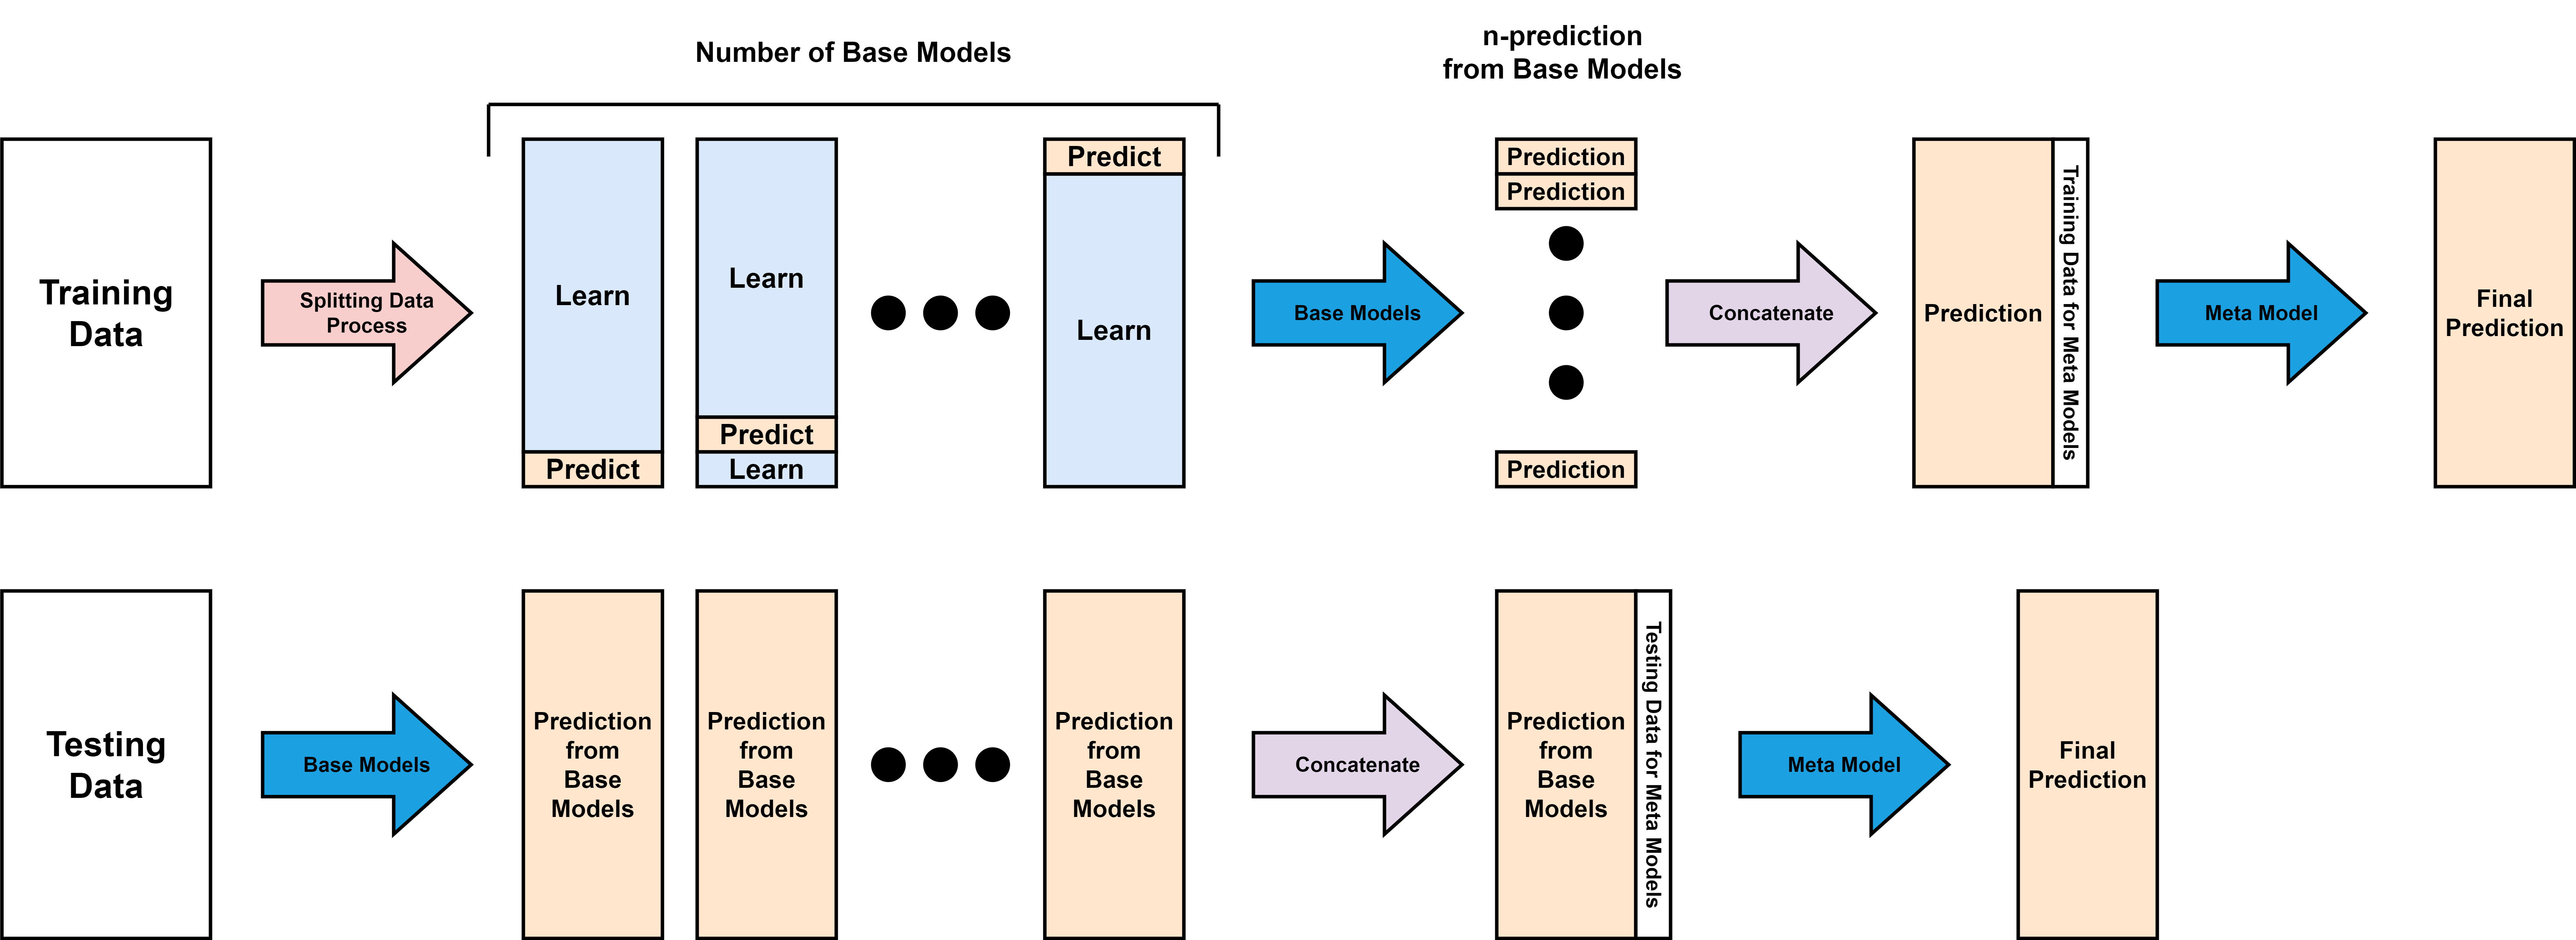
\includegraphics[width=\textwidth]{figures/Fig1.png}
    \caption{Error Based Accumulation Regression Overall Architecture}
    \label{fig:1}
\end{figure}

The 'EBAR' model consists of two fundamental processes: training and prediction. In the training process, a meta-model is chosen to amalgamate results from 9 base models, employing out-of-folds predictions from the base models to construct features for training the meta-model.

The training process is described as follows:
\begin{enumerate}
\item Utilize k-folds cross-validation to partition the training dataset into k non-overlapping subsets, with each subset:
    \begin{enumerate}
        \item Serving as the holdout set.
        \item The remaining data is used for training.
    \end{enumerate}
This data splitting process is depicted in Figure \ref{fig:4}.
\item Train the base models on each training subset and evaluate their performance on the corresponding holdout subset. 
\item Use the predictions from the evaluation (out-of-folds predictions) as input, and the target values as output, to train the higher-order model (meta-model).
\end{enumerate}
\hspace{0.5cm} The prediction process is carried out as follows:
\begin{enumerate}
    \item Collect predictions from all base models on the testing data and use them as meta-features.
    \item Employ these meta-features with the meta-model to make the final predictions.
\end{enumerate}
\hspace{0.5cm} The training and prediction processes are described in Algorithm \ref{alg: Algorithm 1} and Algorithm \ref{alg: Algorithm 2}, and respectively illustrated in Figures \ref{fig:5} and \ref{fig:6}.

\begin{figure}
    \centering
    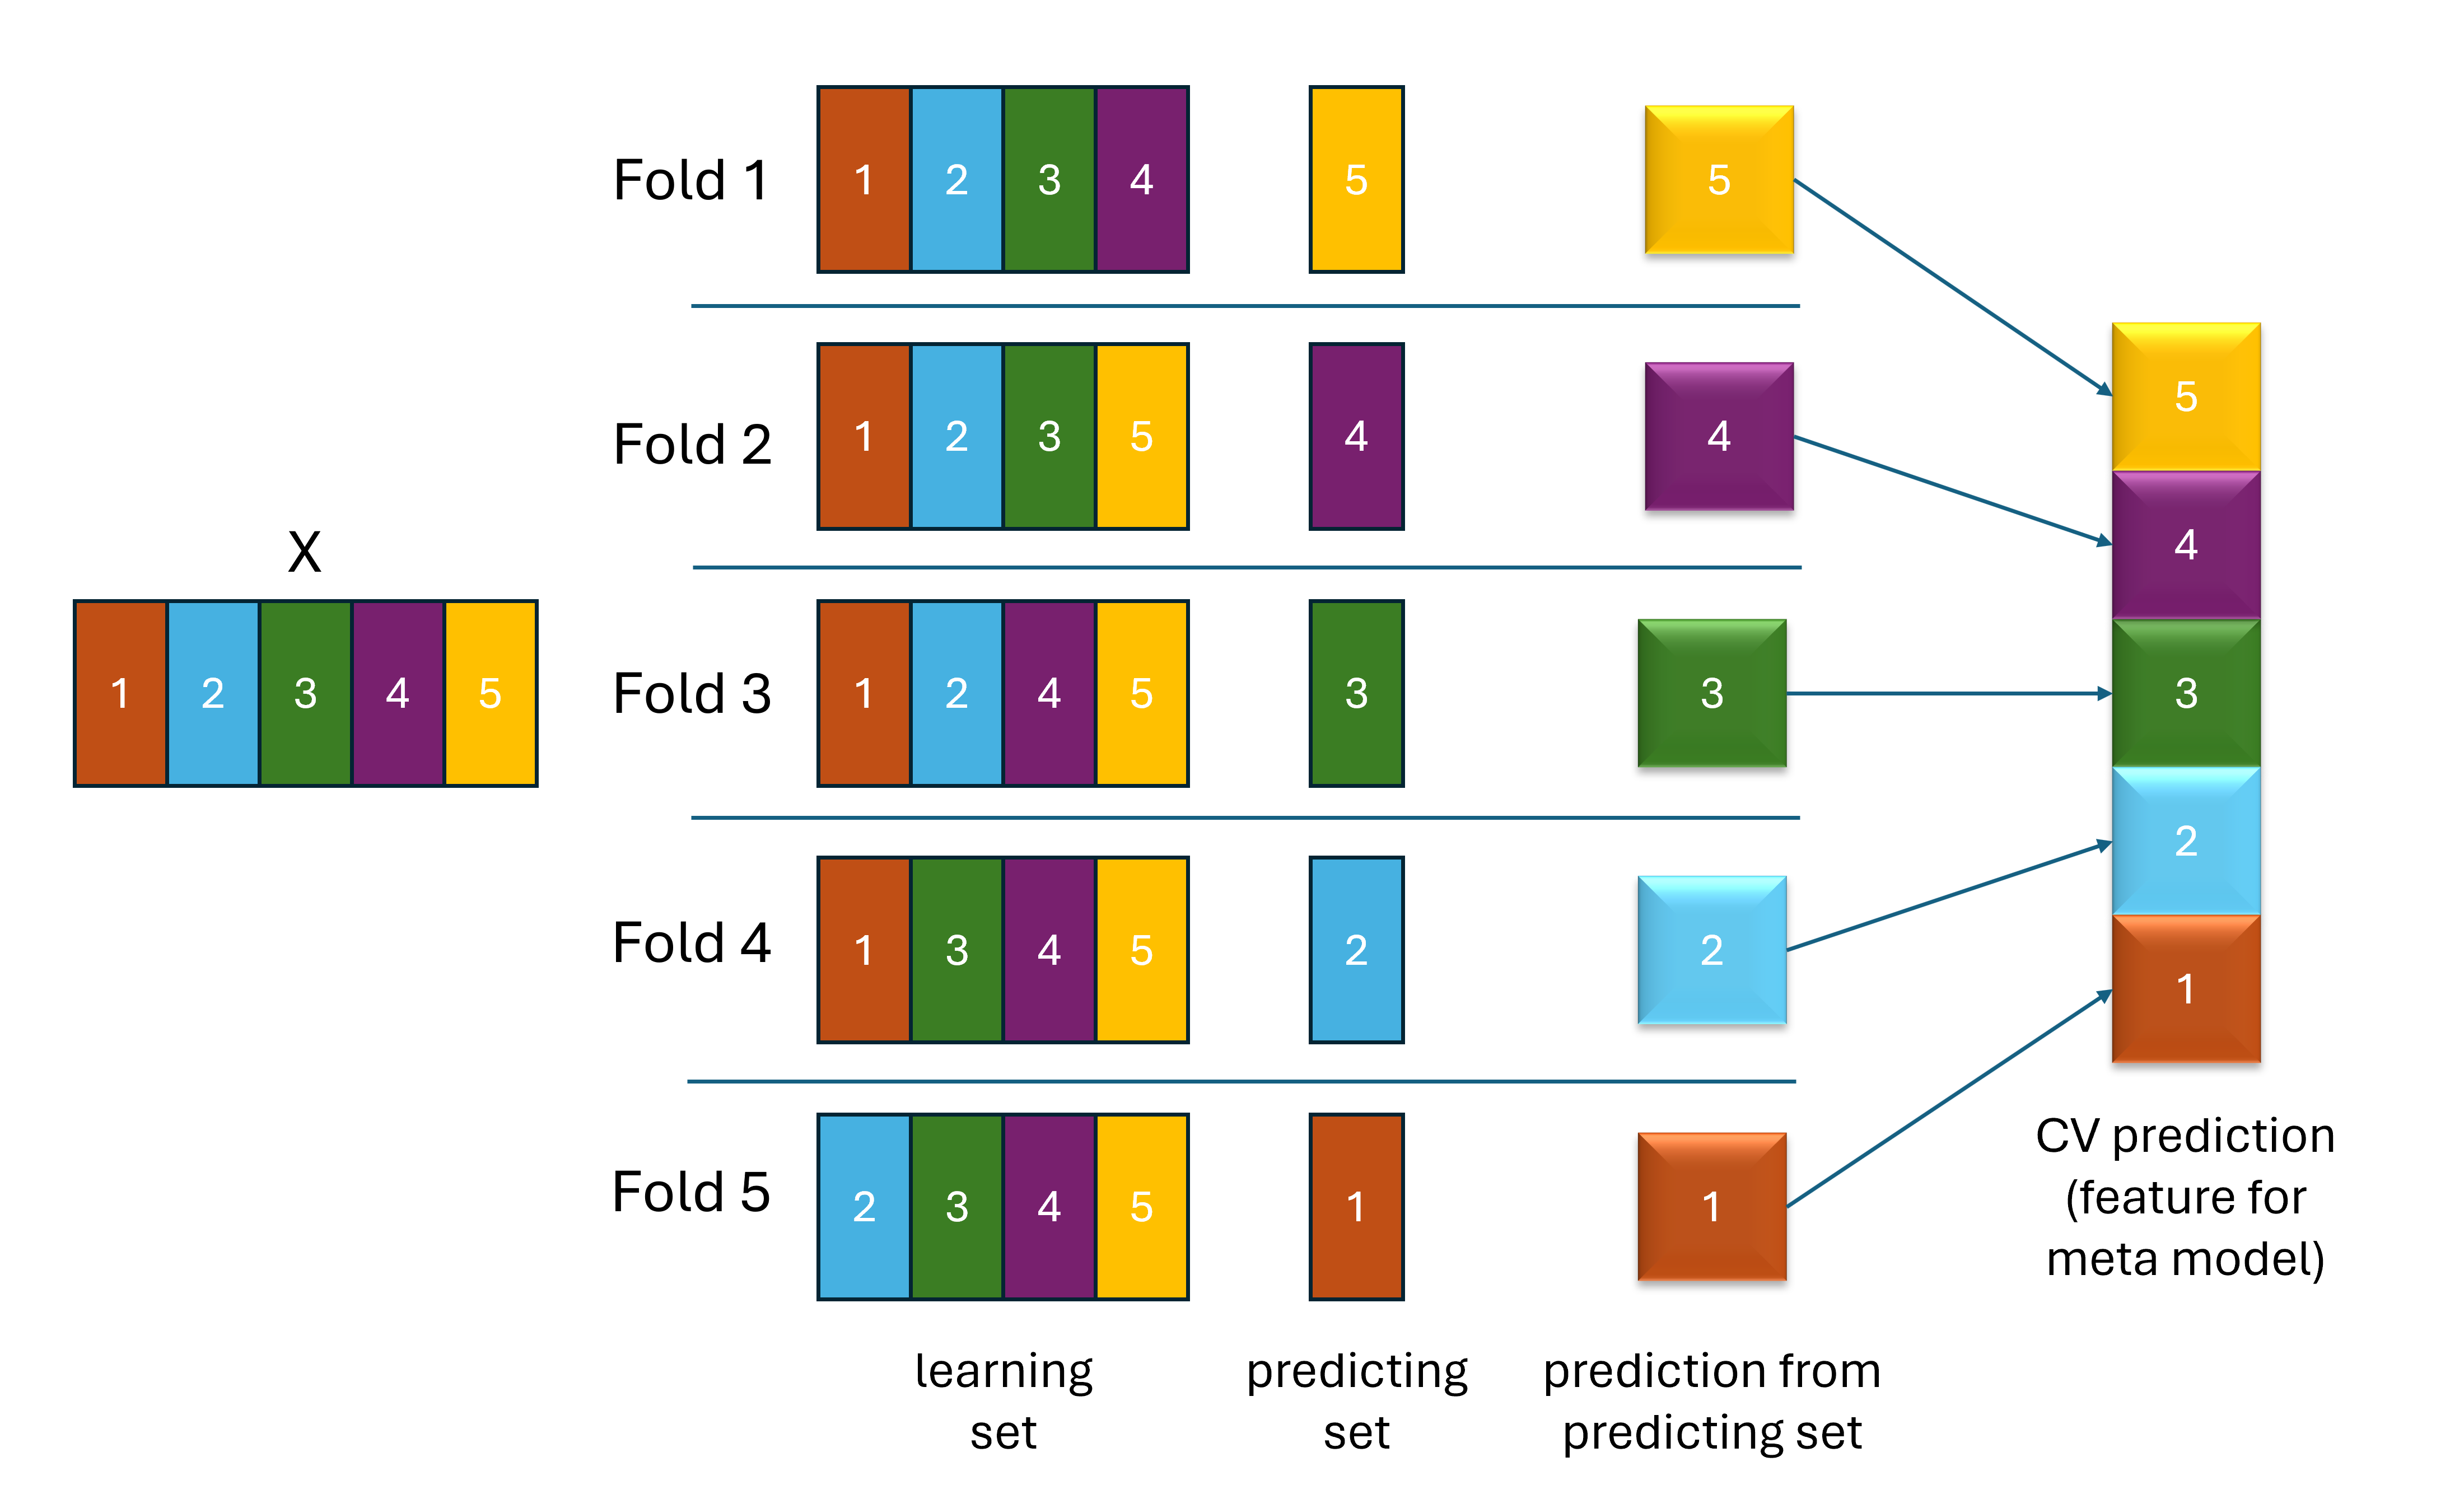
\includegraphics[width=\textwidth]{figures/Picture4.png}
    \caption{Splitting Data Process with $k=5$}
    \label{fig:4}
\end{figure}

\begin{figure}
    \centering
    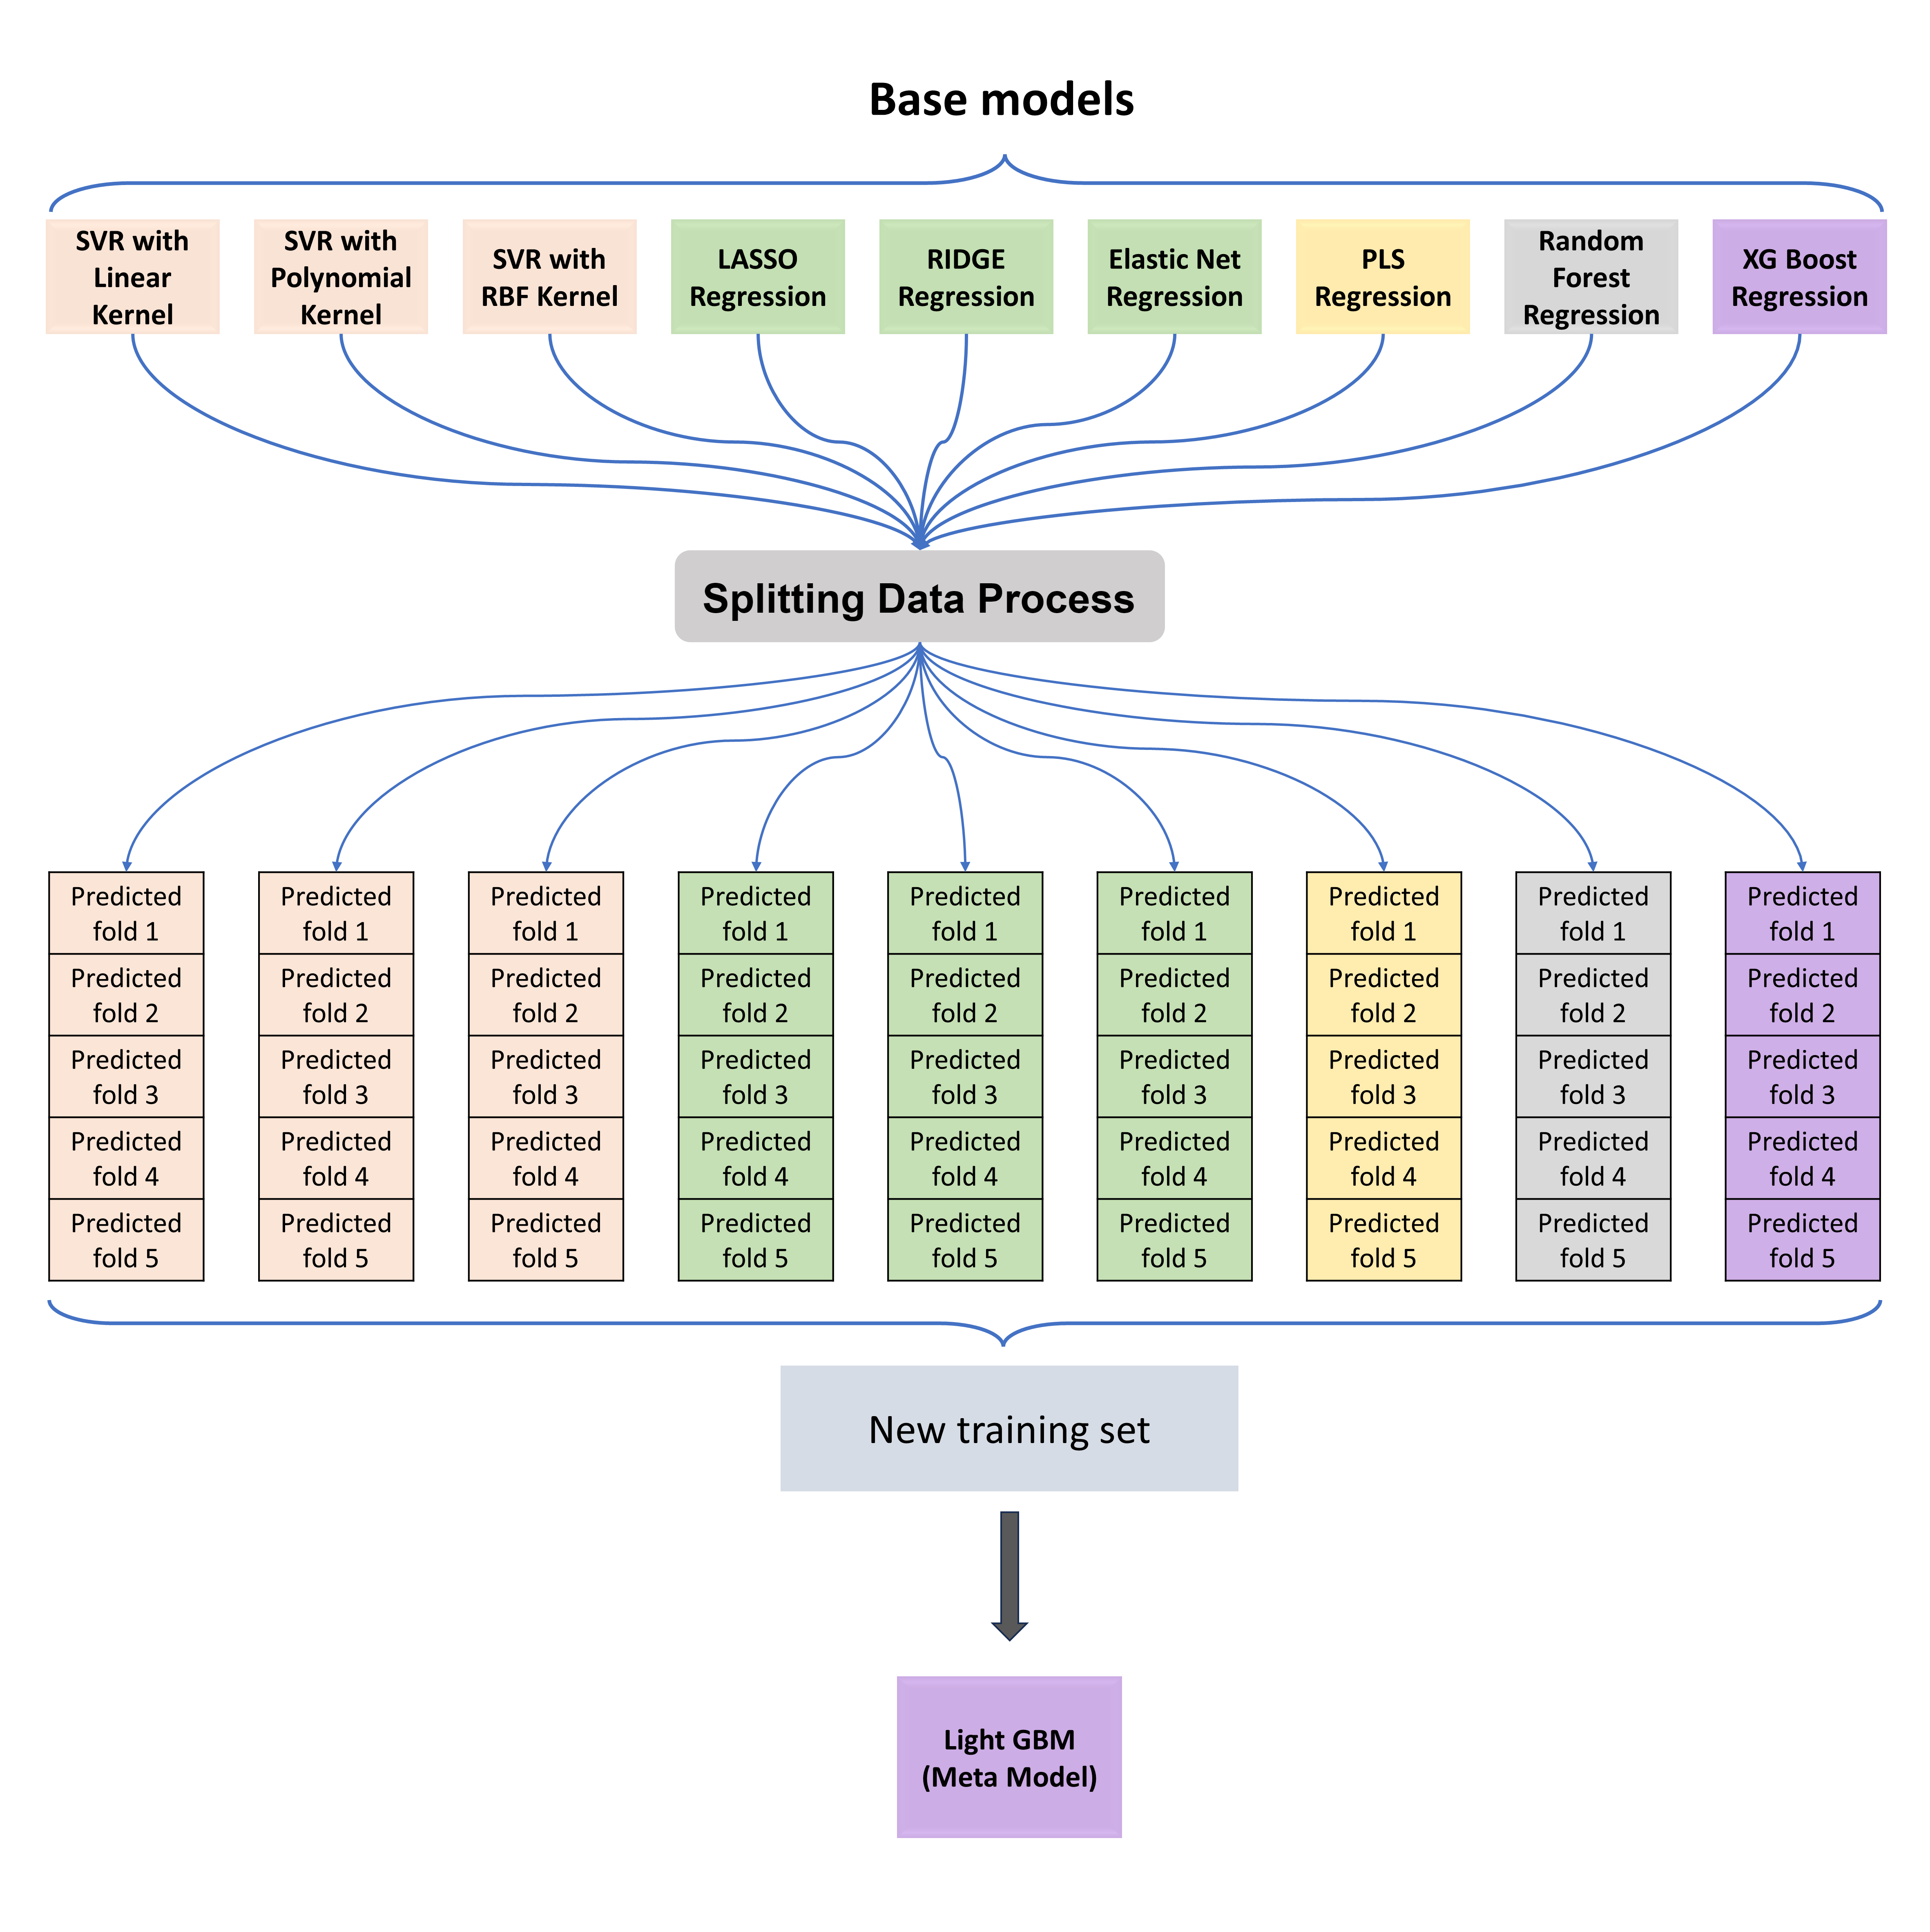
\includegraphics[width=\textwidth]{figures/training.png}
    \caption{Training Strategy}
    \label{fig:5}
\end{figure}

\begin{figure}
    \centering
    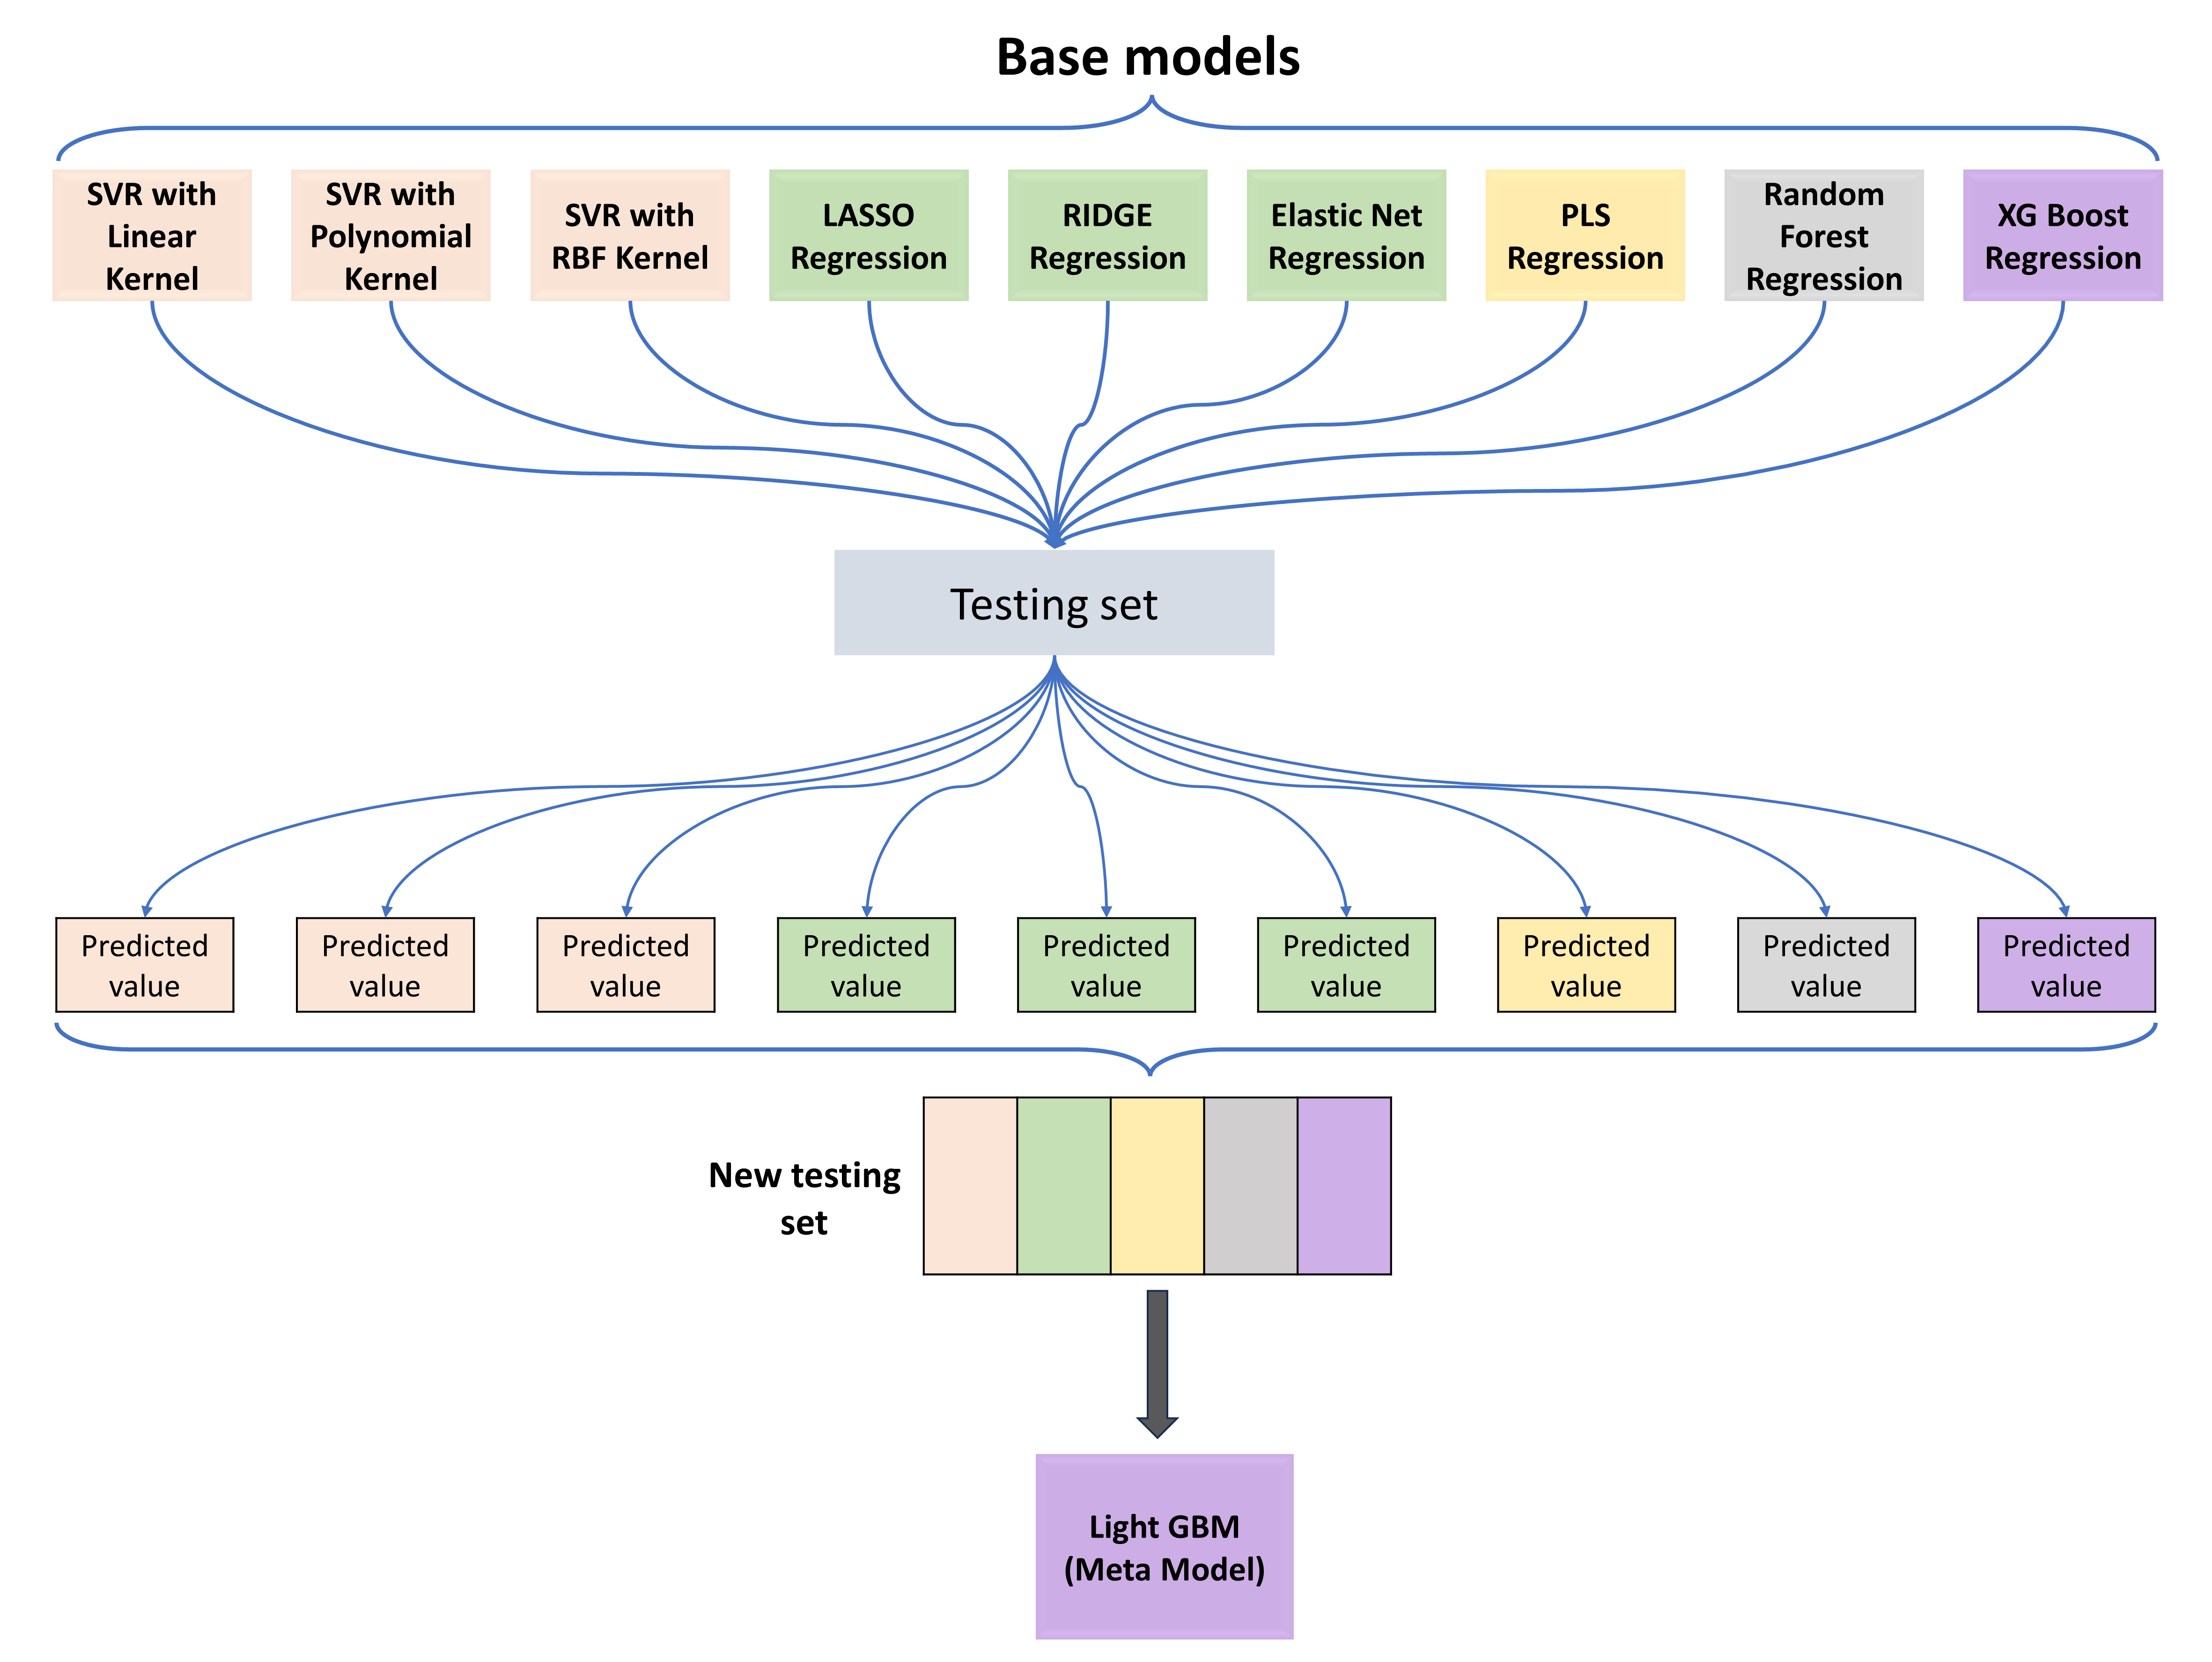
\includegraphics[width=\textwidth]{figures/testing.png}
    \caption{Testing Strategy}
    \label{fig:6}
\end{figure}


\begin{algorithm}[ht]
\footnotesize
\caption{Training Strategy}
\label{alg: Algorithm 1}
        \textbf{Input:} \\
        \hspace*{\algorithmicindent} {$X, y$: data used for training} \\
        \hspace*{\algorithmicindent} {$Bases:$ list of base models in EBAR model} \\
        \hspace*{\algorithmicindent} {$Meta:$ meta model in EBAR model}\\
        \textbf{Parameters:} {$n_{folds} \leftarrow$ number of folds} \\
        \textbf{Output:} \textit{Parameters of models}
	\begin{algorithmic}[1]
            \State Let $features = [ ]$
            \State $KFold \leftarrow$ k-folds cross validation 
		\For {$model$ in $Bases$}
			\For {$idx_{train}, idx_{holdout}$ in $KFold(X, y)$}
				\State $model.fit(X[idx_{train}], y[idx_{train}])$
                \State $pred \leftarrow\ model.predict(X[idx_{holdout}])$
                \State $features.append(pred)$
			\EndFor
		\EndFor
		\State $Meta.fit(features, y)$
	\end{algorithmic} 
\end{algorithm}
\begin{algorithm}[ht]
\footnotesize
\caption{Testing Strategy}
\label{alg: Algorithm 2}
        \textbf{Input:} \\
        \hspace*{\algorithmicindent} {$X, y$: data used for testing} \\
        \hspace*{\algorithmicindent} {$Bases:$ list of base models in EBAR model} \\
        \hspace*{\algorithmicindent} {$Meta:$ meta model in EBAR model}\\
        \textbf{Output:} \textit{Predictions}
	\begin{algorithmic}[1]
            \State Let $features = [ ]$
		\For {$model$ in $Bases$}
                \State $pred \leftarrow\ model.predict(X)$
                \State $features.append(pred)$
		\EndFor
            \State $Predictions \leftarrow\ Meta.predict(features)$
	\end{algorithmic} 
\end{algorithm} 
\subsection{Elimination of Unimportant Wavelengths (Backward Elimination)}

The absorbance data of the samples at various wavelengths are discretized into absorbance values at specific wavelengths denoted as {\(x_1,x_2,…,x_n\)}, which serve as the features in the feature selection problem. Then, the correlation coefficient between each feature and the target variable is computed. Specifically, for \(\textbf{X}_i\) representing the absorbance of samples at wavelength \textit{i}, \textbf{Y} representing the quantity of a substance in the sample, and E denotes the expected value, the correlation coefficient is calculated using the formula (\ref{eq7}):
\begin{equation} \label{eq7}
r_i = \frac{\mathbb{E}[\textbf{X}_i\textbf{Y}] - \mathbb{E}[\textbf{X}_i]\mathbb{E}[\textbf{Y}]}{\sqrt{\mathbb{E}[\textbf{X}_i^2] - (\mathbb{E}[\textbf{X}_i])^2}\sqrt{\mathbb{E}[\textbf{Y}^2] - (\mathbb{E}[\textbf{Y}])^2}}
\end{equation}

\begin{algorithm}[!ht]
    \footnotesize
	\caption{Backward Elimination}
    \label{alg: Algorithm 3}
        \textbf{Input:} \\
        \hspace*{\algorithmicindent} {$X$: feature data of samples} \\
        \hspace*{\algorithmicindent} {$Y$: target data of samples} \\
        \hspace*{\algorithmicindent} {$n_{features}$: number of features} \\
        \hspace*{\algorithmicindent} $S = \{x_{1}, x_{2}, ... , x_{n_{features}}\}$: set of features
        
        \hspace*{\algorithmicindent} {$model:$ model used to eliminate feature} \\
        \textbf{Parameters:} $\alpha \leftarrow$ threshold to eliminate feature \\
        \textbf{Output:} \textit{Set of significant features}
	\begin{algorithmic}[1]
            \State \textit{Let r = dictionary()}
            \State \textit{Let $E_0 = []$}
            \State \textit{Let $E = []$}
            \State \textit{KFold $\leftarrow$ k-folds cross validation} 
		\For {$i=0$ to $n_{features}$}
             \State $r[x_{i}] \leftarrow \rho_{X_{i}, Y}$ 
		\EndFor
        \For {$idx_{train}, idx_{test}$ in $KFold(X, y)$}
			\State $model.fit(X[idx_{train}], y[idx_{train}])$
            \State $Y_{pred} \leftarrow\ model.predict(X[idx_{test}])$
            \State $E_0.append(RMSE(Y_{pred}, Y))$
        \EndFor
        \State $Error_0 \leftarrow\ mean(E_0)$ 
        \State \(r \leftarrow r.sort(ascending)\)
            \For {$x$ in $r.keys()$}
                \State $S \leftarrow S-x$
                \State Delete data column of $X$ corresponding to feature $x$
                \For {$idx_{train}, idx_{test}$ in $KFold(X, y)$}
			         \State $model.fit(X[idx_{train}], y[idx_{train}])$
                      \State $Y_{pred} \leftarrow\ model.predict(X[idx_{test}])$
                      \State $E.append(RMSE(Y_{pred}, Y))$
                \EndFor
                \State $Error \leftarrow\ mean(E)$ 
                \State $p \leftarrow |Error - Error_{0}|/std_{y}$ 
                \If{$p >= \alpha$}
                    \State $S \leftarrow S+x$
                    \State \textbf{break}
                \EndIf
            \EndFor
	\end{algorithmic} 
\end{algorithm}

Subsequently, the wavelengths are ranked in descending order based on their absolute correlation coefficient values. Then, wavelengths with low correlation are systematically removed, and following each removal, the EBAR model in combination with cross-validation is applied to assess the impact of the elimination. The evaluation process unfolds as follows:
\begin{enumerate}
    \item Determine the Root Mean Square Error value \(\textit{Error}_0\) of the EBAR model on the dataset without feature elimination. 
    \item Calculate the Root Mean Square Error value \textit{Error} of the EBAR model on the dataset with feature elimination.
    \item With \(\textit{std}_y\) as the standard deviation of the target variable, calculate the significance level of feature elimination for the model using the formula:
    \[p = \frac{|\textit{Error} - \textit{Error}_0|}{\textit{std}_y}\]
    \item Compare this significance level with the threshold \(\alpha\):
    \begin{enumerate}
        \item If \(p < \alpha\), continue removing the next feature;
        \item If \(p \ge \alpha\), stop the process and retain the last removed feature.
    \end{enumerate}
\end{enumerate}
\hspace{0.5cm} The remaining set of features consists of the wavelengths with the strongest absorbance characteristics. This process is depicted through Algorithm \ref{alg: Algorithm 3}.

\section{Implementation and Results}
\subsection{Dataset}
The dataset used in this study was collected by Gogé et al. \cite{goge2021dataset}, consisting of 196 samples of cattle manure and 136 samples of poultry manure, totaling 332 samples from farming regions in France and Réunion Island. The initial manure samples underwent immediate cryopreservation upon collection to minimize microbial activity affecting \(NH_4\) content. Subsequently, these samples were ground using a Blixer Dito K45 grinder. The samples were then dried at 40°C for four days and ground to a 1 mm particle size using a Cyclotec 1093 mill.

Chemical analysis was undertaken on the manure samples, encompassing dry matter (\(DM\)), ammonium nitrogen (\(NH_4\)), nitrogen (\(N\)), phosphorus pentoxide (\(P_2O_5\)), calcium oxide (\(CaO\)), magnesium oxide (\(MgO\)), and potassium oxide (\(K_2O\). The chemical analysis was performed using an Inductively Coupled Plasma machine (Element XR Thermo Scientific). To reduce research costs, the researchers conducted exhaustive chemical analysis only on \(DM\), \(N\), and \(NH_4\) in all samples, while for the other compounds, they conducted analysis on 158 samples. A detailed exposition of the statistical characteristics of the compound concentrations is provided in Table \ref{tab:table1}.
\renewcommand{\arraystretch}{1.5}
\setlength{\tabcolsep}{4pt}
\begin{table}[!ht]
    \centering
    \begin{tabular}{ccccccc}
        \hline
        \textbf{Compound} & \textbf{n} & \textbf{Mean} & \textbf{SD} & \textbf{Min} & \textbf{Max} & \textbf{Range} \\
        \hline
        \(DM\) & 332 & 37.28 & 20.26 & 11.25 & 82.48 & 71.22 \\
        \(NH_4\) & 332 & 0.262 & 0.276 & 0.001 & 1.086 & 1.085 \\
        \(N\) & 332 & 1.36 & 1.09 & 0.25 & 4.15 & 3.90 \\
        \(CaO\) & 158 & 0.57 & 0.56 & 0.09 & 3.11 & 3.01 \\
        \(K_2O\) & 158 & 1.02 & 0.65 & 0.19 & 3.84 & 3.66 \\
        \(MgO\) & 158 & 0.23 & 0.19 & 0.06 & 1.05 & 0.99 \\
        \(P_2O_5\) & 158 & 0.48 & 0.58 & 0.09 & 3.02 & 2.93 \\
        \hline
    \end{tabular}
    \caption{Statistical Analysis of Compound Concentrations in Samples ( \% of mass)}
    \label{tab:table1}
\end{table}

During the near-infrared (NIR) spectroscopy analysis, the specimens underwent scanning using one of three spectrophotometers: XDS-CIRAD, XDS-ARVALIS, and NIRFlex-LDAR, spanning a spectral range from 1100 to 2500 nm. Each measurement represented the average of 32 scans and was recorded as absorbance (Abs) using the formula: \(Abs=-log⁡(Reflectance)\). NIR spectra for the 196 cattle manure samples and 136 poultry manure samples are presented in Figure \ref{fig:figure5}. Furthermore, Figure \ref{fig:figure7} illustrates the distribution of chemical compound data.
\begin{figure}[ht]
    \centering
    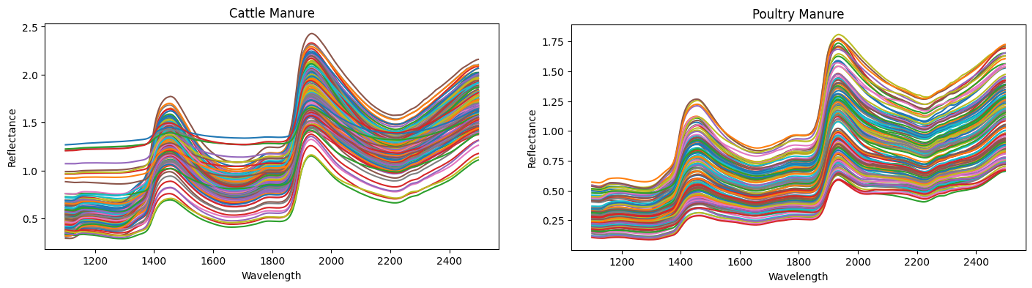
\includegraphics[width=\linewidth]{figures/Picture5.png}
    \caption{NIR Spectra of Cattle Manure}
    \label{fig:figure5}
\end{figure}

\begin{figure}[ht]
    \centering
    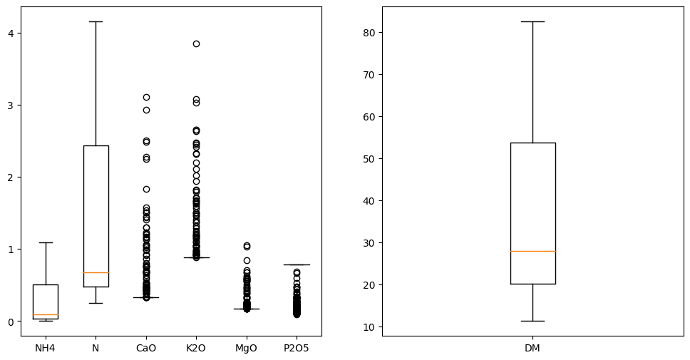
\includegraphics[width=\linewidth]{figures/Picture7.png}
    \caption{Distribution of Chemical Compound Data}
    \label{fig:figure7}
\end{figure}

\subsection{Data Preprocessing}
The dataset was standardized to achieve a mean of 0 and a standard deviation of 1.  NIR spectra of the cattle and poultry manure samples are delineated in Figure \ref{fig:figure8}, while Figure \ref{fig:figure10} presents the distribution of chemical compound data after standardization.

\begin{figure}[ht]
    \centering
    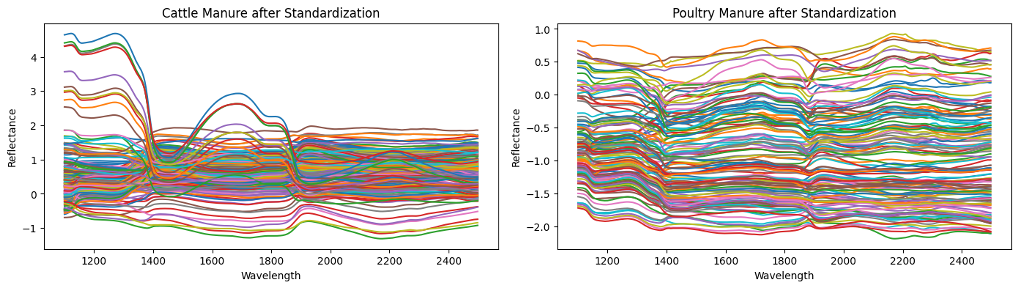
\includegraphics[width=\linewidth]{figures/Picture8.png}
    \caption{Standardized NIR Spectra of Cattle Manure}
    \label{fig:figure8}
\end{figure}

\begin{figure}[ht]
    \centering
    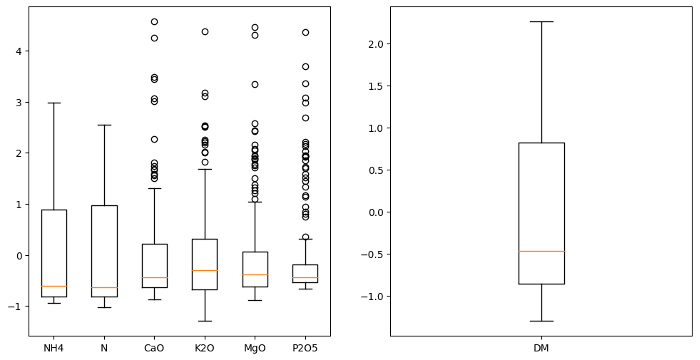
\includegraphics[width=0.8\linewidth]{figures/Picture10.png}
    \caption{Distribution of Chemical Compound Data after Standardization}
    \label{fig:figure10}
\end{figure}

\subsection{Implementation Details}
Hardware: The machine learning models were trained on a system with a CPU (Intel Xeon @2.30 GHz), 13 GB RAM, a Tesla K80 accelerator with 12GB GDDR5 VRAM, and cloud-based TPUs with a computational power of 180 teraflops.

Training Strategy: The training process was orchestrated employing 9 base learner models, including SVR (Linear kernel), SVR (Polynomial kernel), SVR (Radial Basis Function kernel), RIDGE Regression, LASSO Regression, ENET Regression, Random Forest Regression, PLS Regression, and XGBoost Regression. The LightGBM Regression model was used as the meta-model for the EBAR model.

Hyperparameter tuning was performed to determine optimal hyperparameter sets for each model using the Gridsearch method \cite{liashchynskyi2019grid}, the optimal hyperparameters are showed in Table \ref{tab:table2}. The effectiveness of the 11 models was assessed through k-fold cross-validation \cite{van2023plantkvit} with $k=5$. The entire dataset is divided equally into 5 non-overlapping subsets. When running an evaluation, each of the 5 subsets is used as the testing set, and the rest are used as the training sets. The evaluation results of the model are averaged after 5 evaluations.

\renewcommand{\arraystretch}{1.5}
\setlength{\tabcolsep}{4pt}
\begin{table}
    \centering
    \begin{tabular}{ccccc}
        \hline
        \textbf{Algorithm} & \textbf{Parameters} & \textbf{Minimum} & \textbf{Maximum} & \textbf{Optimal} \\
        \hline
        SVR (Linear) & cost (C) & $9.77 \times 10^{-4}$ & 32 & 0.01 \\
                     & margin (epsilon) & 0 & 0.2 & 0.05\\
        \hline
        SVR (Polynomial) & cost (C) & $9.77 \times 10^{-4}$ & 32 & 0.01 \\
                         & degree & 1 & 5 & 4 \\
                         & scale\_factor (scale) & $10^{-10}$ & 0.1 & 0.01 \\
                         & margin (epsilon) & 0 & 0.2 & 0.05 \\
        \hline
        SVR (RBF) & cost (C) & $9.77 \times 10^{-4}$ & 32 & 0.01 \\
                  & rbf\_sigma (sigma) & $10^{-10}$ & 0.1 & 0.05 \\
                  & margin (epsilon) & 0 & 0.2 & 0.05 \\
        \hline
        LASSO & penalty & $10^{-10}$ & 1 & 0.63 \\
              & mixture (alpha) & 1 & 1 & 1 \\
        \hline
        RIDGE & penalty & $10^{-10}$ & 1 & 0.65 \\
              & mixture (alpha) & 0 & 0 & 0 \\
        \hline
        ENET & penalty & $10^{-10}$ & 1 & 0.62 \\
             & mixture (alpha) & 0.05 & 1 & 0.7 \\
        \hline
        PLS & predictor\_prop & 0 & 1 & 0.6 \\
            & num\_comp & 1 & 4 & 3 \\
        \hline
        Random Forest & tree\_depth & 1 & 15 & 12 \\
                      & n\_trees & 1 & 2000 & 1850 \\
                      & min\_rows & 1 & 40 & 32 \\
        \hline 
        XGBoost & tree\_depth & 1 & 15 & 12 \\
                & n\_trees & 1 & 2000 & 1800 \\
                & learn\_rate (eta) & 0.001 & 0.4 & 0.05 \\
                & early\_stop & 3 & 20 & 5 \\
        \hline 
        LightGBM & tree\_depth & 1 & 15 & 12 \\
                 & n\_trees & 1 & 2000 & 1800 \\
                 & learn\_rate (eta) & 0.001 & 0.4 & 0.05 \\
                 & early\_stop & 3 & 20 & 5 \\
        \hline 
    \end{tabular}
    \caption{Ranges of hyperparameters used in tuning of best results for various machine learning technique}
    \label{tab:table2}
\end{table}


\subsection{Metric}
The evaluation was conducted using 2 metrics: Root Mean Square Error (RMSE) and R-squared (\(R^2\)):~\par
RMSE measures the mean error of predicted values \(\hat{y}_i\), in comparison to actual values \(y_i\) in the test dataset with n data samples. The RMSE calculation is delineated by the formula (\ref{eq8}):
\begin{equation} \label{eq8}
RMSE = \sqrt{\frac{\sum{(y_i-\hat{y_i})^2}}{n}}
\end{equation}
\hspace{0.5cm} \(R^2\), also known as the coefficient of determination, serves to evaluate the congruence between a model and the data. Given \(y_i\) as the actual value, \(\hat{y}_i\) as the predicted value, and \(\bar{y}\) representing the mean value of the target variable, the \(R^2\) value is calculated using the following formula (\ref{eq9}):
\begin{equation} \label{eq9}
R^2=1-\frac{\sum(y_i-\hat{y_i})^2}{\sum(y_i-\bar{y})^2}
\end{equation}

The \(R^2\) value spans a range from 0 to 1, with:
\begin{itemize}
    \item \(R^2=0\): indicating that the model does not explain any variation in the data and is entirely uncorrelated to it;
    \item \(R^2=1\): indicating that the model completely explains all the variations in the data and perfectly fits the data;
    \item \(R^2 \epsilon (0,1)\): signifying the relative degree of fit of the model to the data; the higher the \(R^2\) value, the better the model is at explaining variations in the data.
\end{itemize}
\subsection{Evaluation}
Tables \ref{tab:table3} and \ref{tab:table4} demonstrate that the EBAR model outperforms traditional machine learning models across different compounds: \(DM\), \(NH_4\), \(N\), \(P_2O_5\), \(CaO\), and \(K_2O\). Particularly for \(DM\) and \(NH_4\), the proposed model exhibits significantly superior outcomes (\(RMSE_{DM}=3.785, RMSE_{NH_4}=0.053, R_{DM}^2=0.962,R_{NH_4}^2=0.968\)). However, for \(MgO\), the SVR model with the RBF kernel provides slightly better results with \(RMSE_{SVR(RBF)} =0.078\) and \(R_{SVR(RBF)}^2=0.837\).

\begin{figure}[ht]
    \centering
    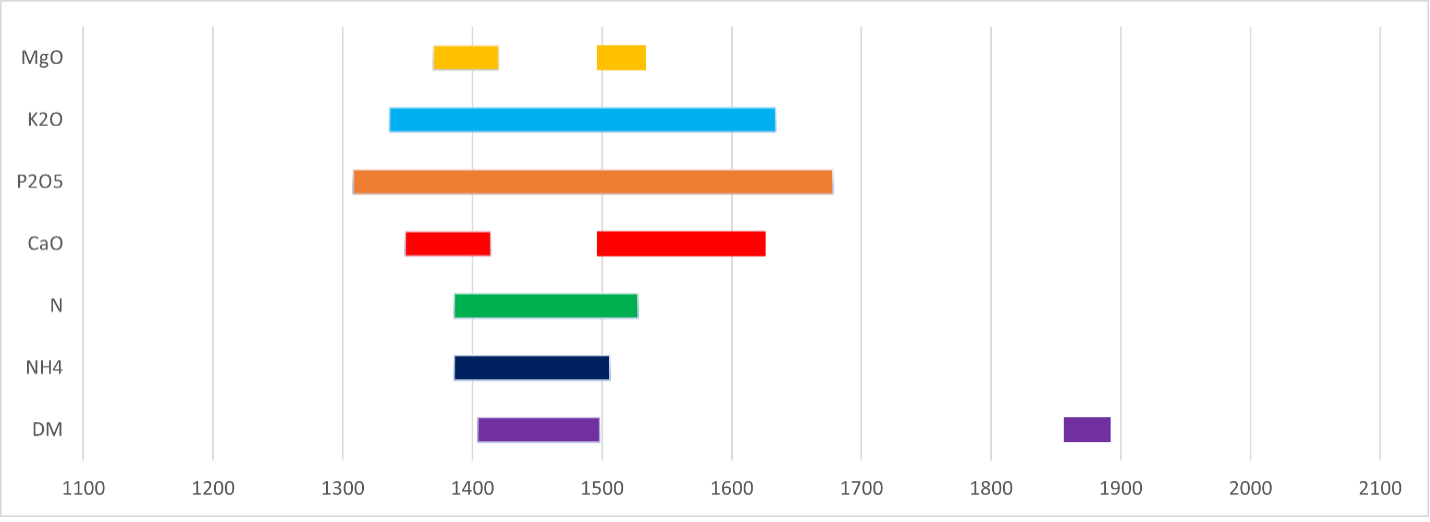
\includegraphics[width=\linewidth]{figures/Picture11.png}
    \caption{Wavelength Ranges of Maximum Absorption for DM, NH4, N, P2O5, CaO, MgO, and K2O}
    \label{fig:figure11}
\end{figure}

Figure \ref{fig:figure11} illustrates the wavelength ranges at which each constituent in the sample exhibits maximum absorption. Specifically, the wavelength range for \(DM\) falls within 1404-1498 and 1856-1892 nm, \(NH_4\) falls within 1386-1506 nm, \(N\) falls within 1386-1528 nm, \(CaO\) ranges from 1348-1414 and 1496-1626 nm, \(K_2O\) ranges from 1336-1634 nm, \(P_2O_5\) ranges from 1308-1678 nm, and \(MgO\) ranges from 1370-1420 and 1496-1534 nm. Table \ref{tab:table5} demonstrates that this proposed method successfully identified the absorption maxima wavelengths for \(DM\), \(NH_4\), \(N\), \(K_2O\), and \(P_2O_5\). In the case of \(CaO\) and \(MgO\), the identified wavelength ranges did not converge, indicating that their absorption spectra do not fall within the observed spectral region, which is in accordance with theoretical expectations.
\renewcommand{\arraystretch}{1.5}
\setlength{\tabcolsep}{4pt}
\begin{table}[!ht]
    \small
    \centering
    \begin{tabular}{|c|c|c|c|c|c|c|c|c|}
        \hline
        \textbf{Model} & \textbf{\(DM\)} & \textbf{\(NH_4\)} & \textbf{\(N\)} & \textbf{\(P_2O_5\)} & \textbf{\(CaO\)} & \textbf{\(MgO\)} & \textbf{\(K_2O\)} & \textbf{Average} \\
        \hline
        SVR (Linear) & 6.909 & 0.075 & 0.343 & 0.306 & 0.332 & 0.096 & 0.399 & 1.209 \\ \hline
        SVR (Polynomial) & 5.158 & 0.078 & 0.346 & 0.307 & 0.410 & 0.091 & 0.398 & 0.970 \\ \hline
        SVR (RBF) & 5.005 & 0.091 & 0.252 & 0.275 & 0.373 & \textbf{0.078} & 0.374 & 0.921 \\ \hline
        LASSO & 7.154 & 0.082 & 0.368 & 0.317 & 0.335 & 0.091 & 0.412 & 1.251 \\ \hline
        RIDGE & 9.307 & 0.102 & 0.505 & 0.390 & 0.394 & 0.107 & 0.472 & 1.611 \\ \hline
        ENET & 7.103 & 0.083 & 0.370 & 0.317 & 0.335 & 0.090 & 0.412 & 1.252 \\ \hline
        PLS & 8.647 & 0.097 & 0.449 & 0.320 & 0.349 & 0.092 & 0.441 & 1.485 \\ \hline
        Random Forest & 5.987 & 0.091 & 0.339 & 0.449 & 0.380 & 0.121 & 0.471 & 1.120 \\ \hline
        XGBoost & 5.642 & 0.082 & 0.279 & 0.458 & 0.407 & 0.133 & 0.414 & 1.059 \\ \hline
        LightGBM & 4.607 & 0.092 & 0.345 & 0.325 & 0.392 & 0.114 & 0.414 & 0.898 \\ \hline
        Proposed Model - EBAR & \textbf{3.785} & \textbf{0.053} & \textbf{0.215} & \textbf{0.264} & \textbf{0.304} & 0.089 & \textbf{0.372} & \textbf{0.726} \\
        \hline
    \end{tabular}
    \caption{RMSE of different models across \(DM\), \(NH_4\), \(N\), \(P_2O_5\), \(CaO\), \(MgO\), and \(K2O\)}
    \label{tab:table3}
\end{table}

\begin{table}[!ht]
    \small
    \centering
    \begin{center}
        % \begin{tabular}{|P{1 in}|P{0.35 in}|P{0.35 in}|P{0.35 in}|P{0.35 in}|P{0.35 in}|P{0.35 in}|P{0.35 in}|P{0.6 in}|}
        \begin{tabular}{|c|c|c|c|c|c|c|c|c|}
        \hline
        \textbf{Model} & \textbf{\(DM\)} & \textbf{\(NH_4\)} & \textbf{\(N\)} & \textbf{\(P_2O_5\)} & \textbf{\(CaO\)} & \textbf{\(MgO\)} & \textbf{\(K_2O\)} & \textbf{Average} \\
        \hline
        SVR (Linear) & 0.919 & 0.944 & 0.928 & 0.770 & 0.673 & 0.716 & 0.656 & 0.801 \\
        \hline
        SVR (Polynomial) & 0.948 & 0.946 & 0.924 & 0.772 & 0.470 & 0.766 & 0.658 & 0.783 \\
        \hline
        SVR (RBF) & 0.950 & 0.896 & 0.951 & 0.852 & 0.564 & \textbf{0.837} & 0.689 & 0.820 \\
        \hline
        LASSO & 0.892 & 0.924 & 0.900 & 0.781 & 0.649 & 0.761 & 0.624 & 0.790 \\
        \hline
        RIDGE & 0.812 & 0.868 & 808 & 0.660 & 0.527 & 0.678 & 0.517 & 0.696 \\
        \hline
        ENET & 0.894 & 0.923 & 0.899 & 0.781 & 0.648 & 0.771 & 0.624 & 0.791 \\
        \hline
        PLS & 0.839 & 0.894 & 0.851 & 0.742 & 0.611 & 0.748 & 0.557 & 0.749 \\
        \hline
        Random Forest & 0.915 & 0.897 & 0.913 & 0.568 & 0.676 & 0.709 & 0.677 & 0.765 \\
        \hline
        XGBoost & 0.924 & 0.916 & 0.937 & 0.658 & 0.552 & 0.612 & 0.729 & 0.761 \\
        \hline
        LightGBM & 0.943 & 0.901 & 0.908 & 0.778 & 0.532 & 0.752 & 0.729 & 0.792 \\
        \hline
        Proposed Model - EBAR & \textbf{0.962} & \textbf{0.968} & \textbf{0.966} & \textbf{0.878} & \textbf{0.741} & 0.799 & \textbf{0.738} & \textbf{0.865} \\
    \hline
    \end{tabular}
    \caption{R-squared of different models across \(DM\), \(NH_4\), \(N\), \(P_2O_5\), \(CaO\), \(MgO\), and \(K2O\)}
    \label{tab:table4}
    \end{center}
\end{table}


\setlength{\tabcolsep}{3pt}
\begin{table}[!ht]
    \centering
    % \begin{tabular}{|P{1.2 in}|P{1.8in}|P{1.8in}|}
    \begin{tabular}{|c|c|c|}
        \hline
        \textbf{Compound} & \textbf{Experimental Wavelength Ranges} & \textbf{Theoretical Wavelength Ranges} \\
        \hline
        \(DM\) & 1404-1498 and 1856-1892 & 1400-1500 and 1800-1900 \\ \hline
        \(NH_4\) & 1386-1506 & 1300-1500 \\ \hline
        \(N\) & 1386-1528 & 1300-1550 \\ \hline
        \(CaO\) & 1348-1414 and 1496-1626 & 550-650 \\ \hline
        \(K_2O\) & 1336-1634 & 1050-1640 \\ \hline
        \(MgO\) & 1308-1678 & 1050-1640 \\ \hline
        \(P_2O_5\) & 1370-1420 and 1496-1534 & 260-330 \\
        \hline
    \end{tabular}
    \caption{Comparison of Experimental and Theoretical Wavelength Ranges}
    \label{tab:table5}
\end{table}

\section{Discussion}
In this study, the EBAR model is proposed, demonstrating a notably improved predictive performance compared to traditional machine learning methods for various chemical components, namely DM, \(NH_4\), N, CaO, MgO, \(P_2O_5\), and \(K_2 O\), in both cattle and poultry fertilizers. Furthermore, when compared to the findings of a previous study by \cite{cobbinah2022using}, the EBAR model exhibits marginally better results, with \(RMSE_{mean}=0.726\) and \(R_{mean}^2=0.865\) for the EBAR model, as opposed to \(RMSE_{mean}=0.772\) and \(R_{mean}^2=0.863\) for the Stacked Regression model. Particularly, in contrast to research employing the PLS model for chemical content prediction, the EBAR model outperforms its predecessor in terms of accuracy.

The proposed Backward Elimination technique narrows down the wavelength range where chemicals in the sample exhibit strong absorption. This determination holds significance not only from a chemical perspective in explaining the chemical interactions but also contributes to refining the machine learning model. This method reduces feature space without compromising prediction accuracy, thus saving training time and model complexity.

In the case of MgO and CaO, while the EBAR model accurately predicts their content, Backward Elimination falters in explaining the precise wavelength range of maximal absorption. This arises from the fact that the observed fertilizer samples are natural products and have not undergone chemical interventions by humans. Table 1 reveals that the ratio of MgO and CaO to \(P_2O_5\) is approximately 1:3 and 1:1, respectively, in all criteria. Therefore, the EBAR model can predict MgO and CaO based on this ratio. This constraint can be addressed by expanding the surveyed spectral range and examining fertilizer samples that have undergone human chemical interventions.

Further optimization of the EBAR model can be achieved with an extended exploration of hyperparameter selection through Gridsearch Cross Validation. Additionally, the proposed model would exhibit enhanced performance through the augmentation of sample diversity, data distribution, and amount of samples. Henceforth, this study exhibits considerable potential for prospective avenues of future expansion.

\section{Conclusions and Future Work}

The utilization of machine learning techniques has been demonstrated as a reliable method for qualitative and quantitative analysis of NIR spectra in various industrial and agricultural domains. Although substantial prior endeavors have been conducted such as \cite{feng2022evaluation}, \cite{huang2008evaluation}, and \cite{devianti2022near}, this study proposes a synthetic machine learning model named EBAR, derived from traditional machine learning models, specifically designed for the chemical analysis of fertilizer samples. The model's effectiveness is evaluated using RMSE and R-squared metrics, demonstrating its superiority over conventional machine learning models, particularly the PLS model commonly employed in NIR spectroscopy, with \(RMSE_{mean}=0.726\) and \(R_{mean}^2=0.865\). Furthermore, this study introduces a method for determining the wavelength range of maximum absorption for various chemical components, providing a deeper understanding of their interaction with light and electromagnetic waves and furthering model development.

The results of this study are promising for numerous potential real-world applications. In the future, research efforts will be concentrated on the expansion of the dataset to encompass a broader data distribution, enriching fertilizer samples with human-induced chemical interactions, and extending the surveyed wavelength range to ensure accurate identification of maximum absorption wavelengths for each component. Additionally, the research will concentrate on the enhancement of model efficiency. The scope of this research is not limited to fertilizer samples and can be applied to various other types of products such as meat, fish, vegetables, fruits, or any other food items.

\begin{Acknowledgements}
This study is funded and implemented for the project with number "24/HĐ-SKHCN,2023". This work is supported by the People’s Committee, Da Nang, and the University of Science and
Technology, University of Danang.
\end{Acknowledgements}

\begin{thebibliography}{}{

\fontsize{9pt}{10pt}\selectfont

\bibitem[Almaspoor et al. 2021]{almaspoor2021support} Almaspoor, M. H., Safaei, A., Salajegheh, A., Minaei-Bidgoli, B.: "Support Vector Machines in Big Data Classification: A Systematic Literature Review";  (2021).

\bibitem[Chandrashekar and Sahin 2014]{chandrashekar2014survey} Chandrashekar, G., Sahin, F.: "A survey on feature selection methods"; (2014), Computers \& Electrical Engineering, 40(1), 16–28.

\bibitem[Cobbinah et al. 2022]{cobbinah2022using} Cobbinah, E., Generalao, O., Lageshetty, S. K., Adrianto, I., Singh, S., Dumancas, G. G.: "Using Near-Infrared Spectroscopy and Stacked Regression for the Simultaneous Determination of Fresh Cattle and Poultry Manure Chemical Properties"; (2022), Chemosensors, 10(10), 410.

\bibitem[Cozzolino et al. 2007]{cozzolino2007effect} Cozzolino, D., Liu, L., Cynkar, W. U., Dambergs, R. G., Janik, L., Colby, C. B., Gishen, M.: "Effect of temperature variation on the visible and near infrared spectra of wine and the consequences on the partial least square calibrations developed to measure chemical composition"; (2007), Analytica Chimica Acta, 588(2), 224–230.

\bibitem[Devianti et al. 2021]{devianti2021organic} Devianti, D., Yusmanizar, Y., Syakur, S., Munawar, A. A., \& Yunus, Y: "Organic fertilizer from agricultural waste: determination of phosphorus content using near infrared reflectance"; (2021), IOP Conference Series: Earth and Environmental Science, 644, 012002. IOP Publishing.

\bibitem[Devianti et al. 2022]{devianti2022near} Devianti, D., Sufardi, S., Mustaqimah, M., Munawar, A. A.: "Near Infrared Technology in Agricultural Sustainability: Rapid Prediction of Nitrogen Content from Organic Fertilizer"; (2022), Transdisciplinary Journal of Engineering \& Science, 13.

\bibitem[Dong et al. 2020]{dong2020survey} Dong, X., Yu, Z., Cao, W., Shi, Y., Ma, Q.: "A survey on ensemble learning"; (2020), Frontiers of Computer Science, 14, 241–258.

\bibitem[Feng et al. 2022]{feng2022evaluation} Feng, X., Larson, R. A., Digman, M. F.: "Evaluation of Near-Infrared Reflectance and Transflectance Sensing System for Predicting Manure Nutrients". (2022), Remote Sensing, 14(4), 963.

\bibitem[Fu et al. 2015]{fu2015using} Fu, Y., Li, Z., Zhang, H., Xu, P.: "Using support vector machine to predict next day electricity load of public buildings with sub-metering devices"; (2015), Procedia Engineering, 121, 1016–1022.

\bibitem[Fuquay et al. 2011]{fuquay2011encyclopedia} Fuquay, J. W., McSweeney, P. L. H., Fox, P. F.: "Encyclopedia of dairy sciences"; (2011), Academic Press.

\bibitem[Gogé et al. 2021]{goge2021dataset} Gogé, F., Thuriès, L., Fouad, Y., Damay, N., Davrieux, F., Moussard, G., Morvan, T.: "Dataset of chemical and near-infrared spectroscopy measurements of fresh and dried poultry and cattle manure"; (2021), Data in Brief, 34, 106647.

\bibitem[Hien 2022]{ngo2022deep} Hien, N., L., H.: "Deep Learning Analysis and Optimization for Different Data Sources in Autonomous Vehicles"; (2022), Luleå University of Technology, Department of Computer Science, Electrical and Space Engineering, 130.

\bibitem[Hien et al. 2021]{hien2021keyphrase} Hien, N. L. H., Minh, H. H., Van Tien, N., Van Hieu, N.: "Keyphrase Extraction Model: A New Design and Application on Tourism Information"; (2021), Informatica, 45(4), 563–569.

\bibitem[Hien et al. 2024]{hien2021artwork} Hien, N. L. H., Kor, A.-L., Ang, M. C., Rondeau, E., Georges, J.-P.: "Image Filtering Techniques for Object Recognition in Autonomous Vehicles"; (2024), Journal of Universal Computer Science, 30(1), 49–92.

\bibitem[Hieu et al. 2023]{van2023plantkvit}Van Hieu, N., Hien, N. L. H., Van Huy, L., Tuong, N. H., Thoa, P. T. K.: "PlantKViT: A Combination Model of Vision Transformer and KNN for Forest Plants Classification"; (2023), JUCS: Journal of Universal Computer Science, 29(9).

\bibitem[Horf et al. 2022]{horf2022optical} Horf, M., Vogel, S., Drücker, H., Gebbers, R., Olfs, H.W: "Optical Spectrometry to Determine Nutrient Concentrations and other Physicochemical Parameters in Liquid Organic Manures: A Review"; (2022), Agronomy, 12(2), 514.

\bibitem[Huang et al. 2008]{huang2008evaluation} Huang, G., Han, L., Yang, Z., Wang, X.: "Evaluation of the nutrient metal content in Chinese animal manure compost using near infrared spectroscopy (NIRS)"; (2008), Bioresource Technology, 99(17), 8164–8169.

\bibitem[Huy et al. 2023]{huy2023sentiment} Van Huy, L., Hien, N. L. H., Phuong, N. T. H., Van Hieu, N.: "Deep Learning Model with Hierarchical Attention Mechanism for Sentiment Classification of Vietnamese Comments"; (2023), Cybernetics and Physics, 12(2), 111–120.

\bibitem[Jiaying et al. 2022]{jiaying2022functions} Jiaying, M., Tingting, C., Jie, L., Weimeng, F., Baohua, F., Guangyan, L.: "Functions of nitrogen, phosphorus and potassium in energy status and their influences on rice growth and development"; (2022), Rice Science, 29(2), 166–178.

\bibitem[Jiang and Chen 2019]{jiang2019determination} Jiang, H., Chen, Q.: "Determination of adulteration content in extra virgin olive oil using FT-NIR spectroscopy combined with the BOSS--PLS algorithm"; (2019), Molecules, 24(11), 2134.

\bibitem[Kacprzak et al. 2023]{kacprzak2023cycles}Kacprzak, M., Malińska, K., Grosser, A., Sobik-Szołtysek, J., Wystalska, K., Dróżdż, D., Meers, E.: "Cycles of carbon, nitrogen and phosphorus in poultry manure management technologies--environmental aspects"; (2023), Critical Reviews in Environmental Science and Technology, 53(8), 914–938.

\bibitem[Kumaravelu et al. 2015]{kumaravelu2015review}Kumaravelu, C., Gopal, A.: "A review on the applications of Near-Infrared spectrometer and Chemometrics for the agro-food processing industries"; (2015), 2015 IEEE Technological Innovation in ICT for Agriculture and Rural Development (TIAR), 8–12.

\bibitem[Liashchynskyi and Liashchynskyi 2019]{liashchynskyi2019grid}Liashchynskyi, P., Liashchynskyi, P.: "Grid search, random search, genetic algorithm: a big comparison for NAS"; (2019), arXiv Preprint arXiv:1912. 06059.

\bibitem[MacDonald 2010]{macdonald2010manure} MacDonald, J. M.: "Manure use for fertilizer and for energy: Report to Congress"; (2010), DIANE Publishing.

\bibitem[Mamouei et al. 2020]{mamouei2020comparison}Mamouei, M., Budidha, K., Baishya, N., Qassem, M., Kyriacou, P.: "Comparison of wavelength selection methods for in-vitro estimation of lactate: a new unconstrained, genetic algorithm-based wavelength selection"; (2020), Scientific Reports, 10(1), 16905.

\bibitem[Olivos-Trujillo et al. 2015]{olivos2015assessing}Olivos-Trujillo, M., Gajardo, H. A., Salvo, S., González, A., Muñoz, C.: "Assessing the stability of parameters estimation and prediction accuracy in regression methods for estimating seed oil content in Brassica napus L. using NIR spectroscopy"; (2015), 2015 CHILEAN Conference on Electrical, Electronics Engineering, Information and Communication Technologies (CHILECON), 25–30. IEEE.

\bibitem[Özdemir et al. 2018]{ozdemir2018quantification}Özdemir, İ. S., Dağ, Ç., Özinanç, G., Suçsoran, Ö., Ertaş, E., & Bekiroğlu, S.: "Quantification of sterols and fatty acids of extra virgin olive oils by FT-NIR spectroscopy and multivariate statistical analyses"; (2018), LWT, 91, 125–132.

\bibitem[Pagliari et al. 2020]{pagliari2020animal} Pagliari, P., Wilson, M., He, Z.: "Animal manure production and utilization: Impact of modern concentrated animal feeding operations"; (2020), Animal Manure: Production, Characteristics, Environmental Concerns, and Management, 67, 1–14.

\bibitem[Pavia et al. 2015]{pavia2015introduction} Pavia, D., Donald, L.P., Gary, M.L., George, S.K., James, R.V.: "Introduction to spectroscopy"; (2015), SERBIULA (Sistema Librum 2. 0).

\bibitem[Rahman et al. 2016]{rahman2016effect} Rahman, F., Rahman, M. M., Rahman, G. M., Saleque, M. A., Hossain, A. S., Miah, M. G.: "Effect of organic and inorganic fertilizers and rice straw on carbon sequestration and soil fertility under a rice--rice cropping pattern"; (2016), Carbon Management, 7(1–2), 41–53.

\bibitem[Roggo et al. 2007]{roggo2007review} Roggo, Y., Chalus, P., Maurer, L., Lema-Martinez, C., Edmond, A., Jent, N.: "A review of near infrared spectroscopy and chemometrics in pharmaceutical technologies"; (2007), Journal of Pharmaceutical and Biomedical Analysis, 44(3), 683–700.

\bibitem[Tibshirani et al. 1996]{tibshirani1996regression}Tibshirani, R.: "Regression shrinkage and selection via the lasso"; (1996), Journal of the Royal Statistical Society Series B: Statistical Methodology, 58(1), 267–288.

\bibitem[Wieringen 2015]{van2015lecture}van Wieringen, W. N.: "Lecture notes on ridge regression"; (2015), arXiv Preprint arXiv:1509. 09169.

\bibitem[Yu et al. 2023]{yu2023novel}Yu, H., Li, Y., Du, W., Yang, M., Peng, X., Wang, X., Long, J.: "A Novel Interpretable Ensemble Learning Method for NIR-based Rapid Characterization of Petroleum Products"; (2023), IEEE Transactions on Instrumentation and Measurement.

\bibitem[Zhang et al. 2022]{zhang2022review} Zhang, W., Kasun, L. C., Wang, Q. J., Zheng, Y., Lin, Z.: "A Review of Machine Learning for Near-Infrared Spectroscopy"; (2022), Sensors, 22(24), 9764.

\bibitem[Zou and Hastie 2005]{zou2005regularization}Zou, H., Hastie, T.: "Regularization and variable selection via the elastic net"; (2005), Journal of the Royal Statistical Society Series B: Statistical Methodology, 67(2), 301–320.
}
\end{thebibliography}


\end{document}
